Nello schema in figura sono riportate tutte le entità e le relazioni che compongono la base di dati. In ogni entità sono anche elencati tutti gli attributi che la compongono, comprese le chiavi primarie ed eventuali vincoli di unicità.

I campi marcati con una \texttt{x} sono i campi interessati dalla ristrutturazione tramite NoSQL. Fare riferimento alla descrizione presente nella Seconda Parte, in particolare [\ref{sec:soluzione}].

\begin{figure}[H]
	\centering
	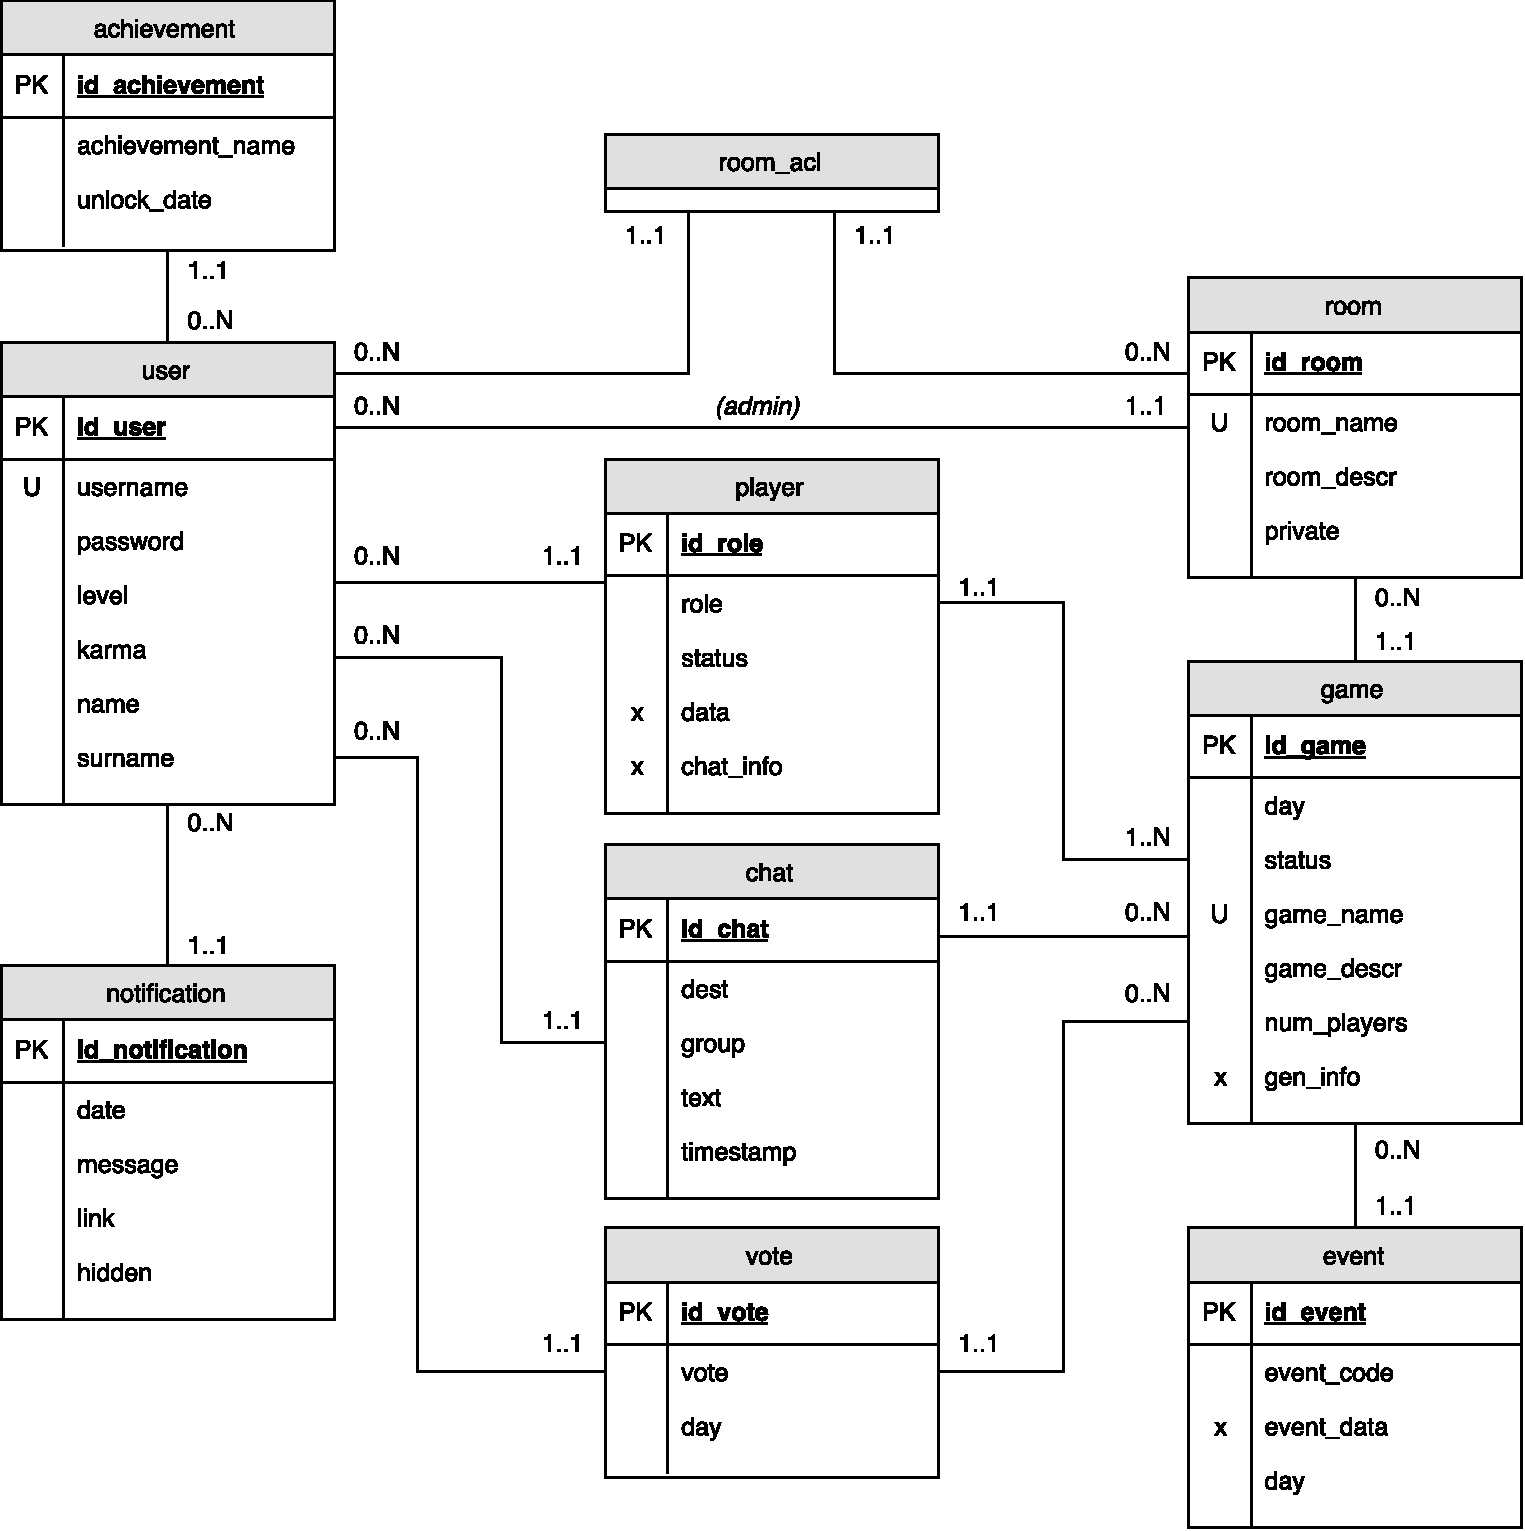
\includegraphics[width=\textwidth]{ER.pdf}
	\caption{Diagramma Entità-Relazione della base di dati}
\end{figure}

